% !TeX root = ../sustechthesis-example.tex

\chapter{基于强化学习的机械狗控制}
在这部分我将阐述关于如何使用强化学习来进行运动控制的内容。相比于传统的基于模型的控制方法,该方法通过在模拟环境中训练控制策略,可以更好地适应复杂的非线性系统动力学和环境不确定性,并且能够实时响应用户命令和环境变化。在这里我们主要关注如何使用强化学习来训练机械狗类型的足式和轮式机器人控制器。

\section[强化学习控制]{强化学习控制}

\subsection[强化学习的基本概念]{强化学习的基本概念\cite{Lee_Bjelonic_Hutter_2023}}

在强化学习中,控制问题被建模为一个马尔可夫决策过程(Markov Decision Process)。MDP是一个RL中常用的用于随机控制过程建模的数学框架,它定义了一个包含状态空间、动作空间、奖励函数和状态转移函数的元组,描述了一个决策过程的基本组成部分。在MDP中,每个时间步骤代理从周围环境中观察到某个状态$s_t \in \mathcal{S}$,并输出一个动作$a_t \in \mathcal{A}$,接着环境通过状态转移函数$p(s_{t+1}|s_t, a_t)$演化到新的状态$s_{t+1}$,并且根据奖励函数给出相应的奖励$r_t\in \mathcal{R}:\mathcal{A}\times\mathcal{S}\to \mathbb{R}$和对更新后的环境状态的观察结果作为下一周期的$s_t$。
代理可以根据$\theta$参数化的随机策略$\pi_\theta(a_t|s_t)$来采取行动。RL通过与环境交互来更新参数$\theta$以最大化累计折扣奖励(cumulative discounted rewards)$\mathbb{E} [\sum_{t=k}^{\infty}\gamma^t r_t]$,其中$k$是当前时间步长(timestep),$\gamma$是折扣因子(discount factor)。

\subsection[基于深度强化学习的控制器的部署和优化流程]{基于深度强化学习的控制器的部署和优化流程}

\begin{enumerate}
    \item 在仿真环境中训练控制器:使用深度强化学习算法在仿真环境中训练控制器,使其能够完成所需的任务。在训练过程中,可以使用特权训练方法来提高训练效率和性能。
    \item 部署控制器到实际环境中:将训练好的控制器部署到实际环境中,例如机器人或移动设备。在实际环境中,控制器将接收传感器数据并输出动作命令。
    \item 优化控制器:在实际环境中,可以使用在线学习方法来进一步优化控制器的性能。例如,可以使用模型预测控制方法来对控制器进行在线微调。
\end{enumerate}

需要注意的是,在实际环境中,传感器数据可能会受到噪声和不确定性的影响,因此需要设计鲁棒性强的控制器来应对这些问题。此外,还需要考虑实际环境中的安全性和可靠性问题。

\section[单层神经网络直接驱动关节方式]{\label{section:direct_network}单层神经网络直接驱动关节方式\cite[p3]{Hwangbo_Lee_Dosovitskiy_Bellicoso_Tsounis_Koltun_Hutter_2019}}


\begin{figure}
    \centering
    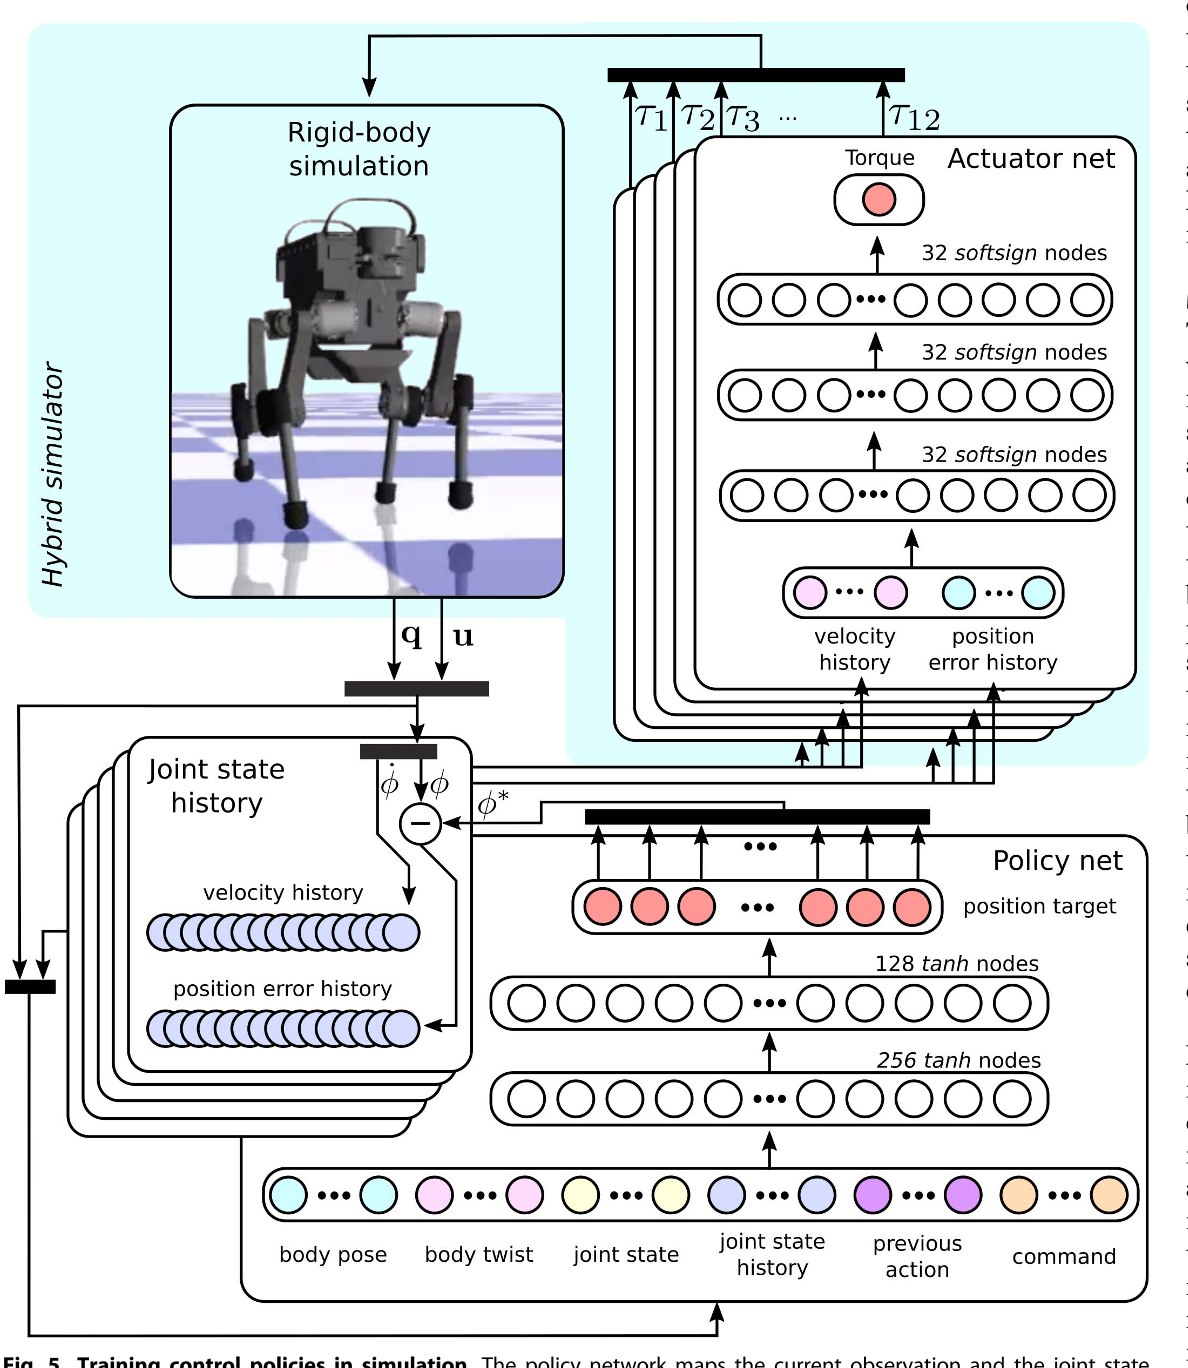
\includegraphics[width=1.0\linewidth]{training_control_policies_in_simulation.png}
    \caption[Training control policies in simulation]{The policy network maps the current joint state and position history to the joint target. }
    \label{fig:training_control_policies_in_simulation}
\end{figure}

如图\ref{fig:training_control_policies_in_simulation}所示,整个训练循环包含下面几个部分:
\begin{itemize}
    \item 首先,一个刚体仿真模拟器运用给定的关节节点扭矩和电流状态计算输出机器人下一状态。与此同时关节点的速度和位置误差在有限时间窗口内被缓冲在节点状态历史中以备网络层使用。
    \item 接着,由两个隐藏层的MLP神经网络构成控制策略,它将输入的电流状态和节点状态历史的观测信息映射成节点位置目标。
    \item 最后,关节点神经网络将关节点状态历史和关节点位置目标映射到$12$个关节点的扭矩值上,然后继续整个循环。
\end{itemize}


\section[双层神经网络本体感知方式]{双层神经网络本体感知方式\cite[p8]{Lee_Hwangbo_Wellhausen_Koltun_Hutter_2020}}

\subsection[总体概况]{总体概况}

\begin{figure}
    \centering
    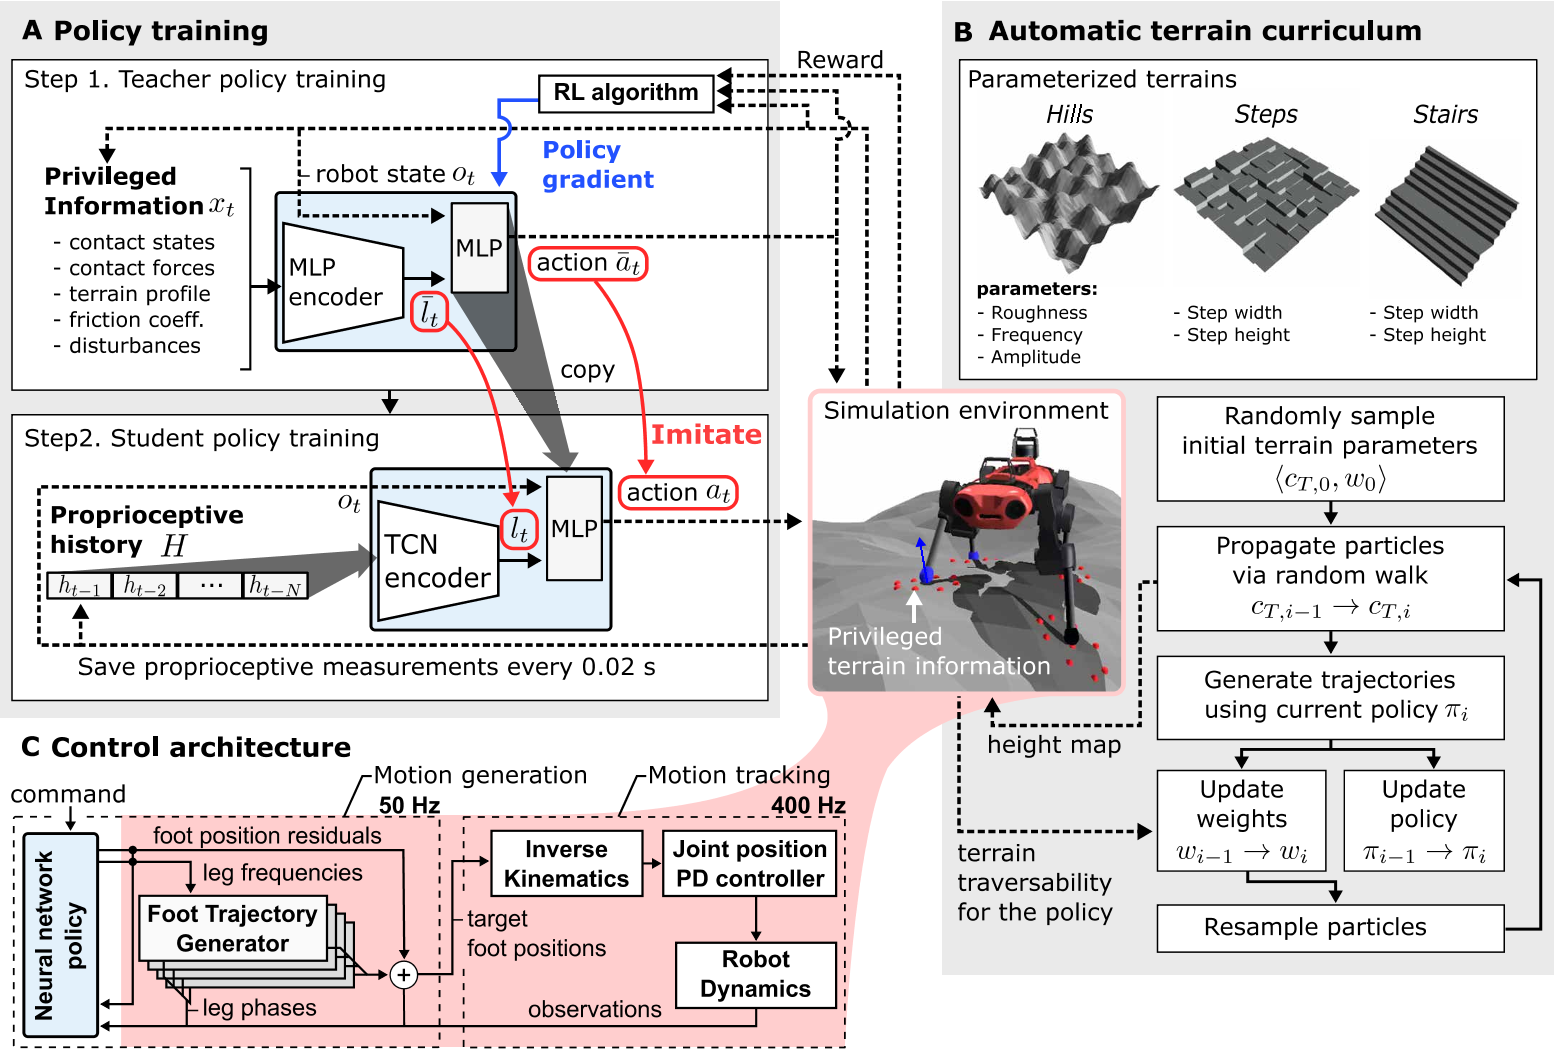
\includegraphics[width=1.0\linewidth]{creating_a_proprioceptive_locomotion_controller.png}
    \caption{Creating a proprioceptive locomotion controller\cite[p7]{Lee_Hwangbo_Wellhausen_Koltun_Hutter_2020}.}
    \label{fig:creating_a_proprioceptive_locomotion_controller}
\end{figure}

  图\ref{fig:creating_a_proprioceptive_locomotion_controller}是一个只采用本体感知进行机器狗控制的RL策略实现架构。它包括训练定义、地形定义、控制架构。
  \begin{itemize}
    \item 策略训练:整个RL训练采用\emph{特权训练(privileged training)}\cite[p]{Chen_Zhou_Koltun_Krähenbühl_2019}的理念,训练过程分为两个阶段,如图\ref{fig:creating_a_proprioceptive_locomotion_controller}A所示。第一阶段用完善的特权信息作为输入训练出一个\emph{教师策略(teacher policy)};第二阶段仅用本体感知作为输入训练出一个\emph{学生策略(student policy)},学生策略的训练过程通过模仿教师策略实现。实际部署到机器人上的策略是学生策略。
    \item 地形定义:RL训练过程是在一定的地形条件下完成的,如图\ref{fig:creating_a_proprioceptive_locomotion_controller}B所示。对于同样的控制命令,不同的地形条件会产生不同的任务难度。为了能更好地促进训练进步,训练过程中的地形采用\emph{自适应地形课程(adaptive terrain curriculum)},它会从简单地形开始根据训练控制器的性能提升而不断提高地形难度,使得RL控制器时钟面对相对于当前状况的中等地形难度。
    \item 控制架构:整个控制架构采用\emph{调节轨迹生成器(Policies Modulating Trajectory Generators, PMTG)\cite[p]{Iscen_Caluwaerts_Tan_Zhang_Coumans_Sindhwani_Vanhoucke_2018}}架构来提供运动生成的先验。神经网络策略通过合成残差位置命令来调节腿相和运动原语,如图\ref{fig:creating_a_proprioceptive_locomotion_controller}C所示。
  \end{itemize}


\subsection[策略训练]{策略训练}
\subsubsection[教师策略]{教师策略}
整个控制问题被构建成一个\emph{马尔科夫决策过程(Markov Decision Process, MDP)}。MDP是一种用于状态和结果部分随机的离散时间控制过程的数学框架。MDP被定义为一个状态空间$\mathcal{S}$,动作空间$\mathcal{A}$,一个标量奖励函数$\mathcal{R}(s_t,s_{t+1})$,一个转移概率$P(s_{t+1}s_t, a_t)$。一个学习代理从策略$\mathbfit{\pi}(a_t|s_t)$中选择一个动作$a_t$并从环境中获得奖励$r_t$。RL的目的是找到一个优化的策略$\mathbfit{\pi}^*$使得无限时间范围内的折扣奖励总和最大。

状态空间$s_t$定义为:$\langle o_t, x_t\rangle$,其中$o_t$是机器人自身的观测信息,$x_t$是特权信息。
\begin{align}
    s_t\begin{cases}
        o_t\begin{cases}
            proprioceptive\ sensors\\
            state\ estimator\begin{cases}
                base\ velocity\\
                orientation\\
            \end{cases}\\
        \end{cases}\\
        x_t\begin{cases}
            only\ for\ simulation
        \end{cases}\\
    \end{cases}
\end{align}

动作空间$\overline a_t$是一个16维向量,由腿的频率和交的位置残差构成。

奖励函数$\mathcal{R}(s_t|s_{t+1})$定义。

\textcolor{red}{reward function definition details ...}

如图\ref{fig:creating_a_proprioceptive_locomotion_controller}A所示,策略网络由两个MLP模块构成。
第一个MLP模块将$x_t$信息转化成潜在向量$\overline{l}_t$,由于$x_t$中并不含有机器人的状态或指令信息,也就是说他只包含地形信息和接触相关的信息。假设$\overline{l}_t$的作用是驱动自适应行为,比如根据地形轮廓改变脚步间隙大小。然后$\overline{l}_t$和$o_t$再提供给第二个MLP网络来计算动作。

训练采用\emph{信任区域策略优化(Trust Region Policy Optimization, TRPO)}\cite[p]{Schulman_Levine_Moritz_Jordan_Abbeel_2015}。

\subsubsection[学生策略]{学生策略}

学生策略仅能获取$o_t$信息。这里的一个关键假设是潜在特征$\overline{l}_t$可以从本体感觉观察的时间序列$h_t$中恢复(部分),$h_t:=o_t\{f_o, joint\ history, previous\ foot\ position\ targets \}$。

学生策略采用TCN\cite[p]{Bai_Kolter_Koltun_2018}编码器。使用TCN架构的原因是它对输入历史长度提供透明的控制,可以容纳长历史,并且已知对超参数设置具有鲁棒性\cite[p]{Bai_Kolter_Koltun_2018}。

学生策略采用监督学习的方式进行训练,损失函数定义为:
\begin{align}
    \mathcal{L}:=(\overline{a}_t(o_t,x_t)-a_t(o_t,H))^2+(\overline{l}_t(o_t, x_t)-l_t(H))^2
\end{align}
带$(\overline{\cdot})$标识的项是来自教师策略的生成。对于每个访问的状态,教师策略计算其嵌入和动作向量$(\overline{\cdot})$,这些教师策略的输出随即被用作与相应状态相关的监督信号。


\subsection[地形定义]{地形定义}
\textcolor{red}{Adaptive terrain curriculum ...}

\subsection[控制架构]{控制架构}

整个控制架构结构如图\ref{fig:creating_a_proprioceptive_locomotion_controller}C所示。它被分为两大类:\emph{运动生成}、\emph{跟随}。整个系统的输入只有\emph{控制指令}和\emph{本体感知},输出为\emph{关节点位置目标}。

运动生成策略是一种基于周期性腿相位的策略,之前的一些工作中通常利用预定义的脚接触时间表\cite[p7]{Bellicoso_Jenelten_Gehring_Hutter_2018,Barasuol_Buchli_Semini_Frigerio_De_Pieri_Caldwell_2013}。为每条腿都定义一个周期的相位变量$\phi_i\in[0.0,2\pi)$。在每一个时间步长$t$里,$\phi_i = (\phi_{i,0}+(f_0+f_i)t)(\mod 2\pi)$,其中$\phi_{i,0}$是初始相位,$f_0$是一般基础频率,$f_i$是第$i$条腿的频率偏移。我们希望腿在$f_0+f_i\neq 0$时表现出周期性运动,并在接触阶段与地面接触。这里基础频率参考之前开发的传统控制\cite[p7]{Bellicoso_Jenelten_Gehring_Hutter_2018}中鹦鹉步态的值,$f_0=1.25$Hz。

\textcolor{red}{target foot position...}

我们采用PMTG架构来将神经网络集成系统中用来调节控制器的输出。整体实现由四个完全相同的\emph{足迹生成器(foot trajectory generators, FTGs)}和一个\emph{神经网络策略(neural network policy, NNP)}构成。足迹生成器是一个输出每条腿的脚位置的函数:$F(\phi):[0.0,2\pi)\to \mathbb{R}^3$。这个FTG在$f_i$不为零时驱动垂直方向的踱步运动。

\begin{note}
\noindent\textcolor{gray}{\small
$F(\phi)$的定义如下:
\begin{align}
    F(\phi_i)=\begin{cases}
        (h(-2k^3+3k^2)-0.5)^{H_i}z &k\in[0,1]\\
        (h(2k^3-9k^2+12k-4)-0.5)^{H_i}z &k\in[1,2]\\
        -0.5^{H_i}z & otherwise\\
    \end{cases}
\end{align}
其中$k=2(\phi_i-\pi)/\pi$,$h$是一个表示最大步高的参数。在摆动相位的每一个阶段都是一个连接最高点和最低点的三次Hermite样条曲线,在连接点处曲线具有一阶连续性(一阶导数为零)。其它的周期函数,如$h_i \sin (\phi_i)$可以用于FTG。给定一组合适的$f_0,h,\phi_{i,0}$参数值,机器人就能稳定地在地面上踱步了。比如,文献\cite[p7]{Lee_Hwangbo_Wellhausen_Koltun_Hutter_2020}中使用的值:$f_0=1.25,h=0.2$,$\phi_{i,0}$从$U(0,2\pi)$中采样得到。}
\end{note}

神经网络策略输出$f_{iS}$和脚的目标位置残差($\Delta \mathbfit{r}_{f_i, T}$)。这样,第$i$个脚的目标位置是$\mathbfit{r}_{f_i, T}:=F(\phi_i)+\Delta \mathbfit{r}_{f_i, T}$。

跟随控制是使用解析\emph{逆运动学(inverse kinematics, IK)}和关节点\emph{位置控制(position control)}实现的。在$H_i$中定义的脚位置首先表述在机器人身体系中,然后用IK计算关节点的位置目标。而关节点的位置目标依靠关节点的PD控制器来跟随。使用IK的好处是可以最大化计算效率同时在\emph{仿真到实际(sim-to-real)}的过程中可以复用已有的位置控制驱动器模型\cite[p]{Lee_Hwangbo_Hutter_2019,Hwangbo_Bellicoso_Fankhauser_Huttery_2016}。

\section[双层网络本体和外部感知融合方式]{双层网络本体和外部感知融合方式\cite[p7]{Miki_Lee_Hwangbo_Wellhausen_Koltun_Hutter_2022}}


\begin{figure}
    \centering
    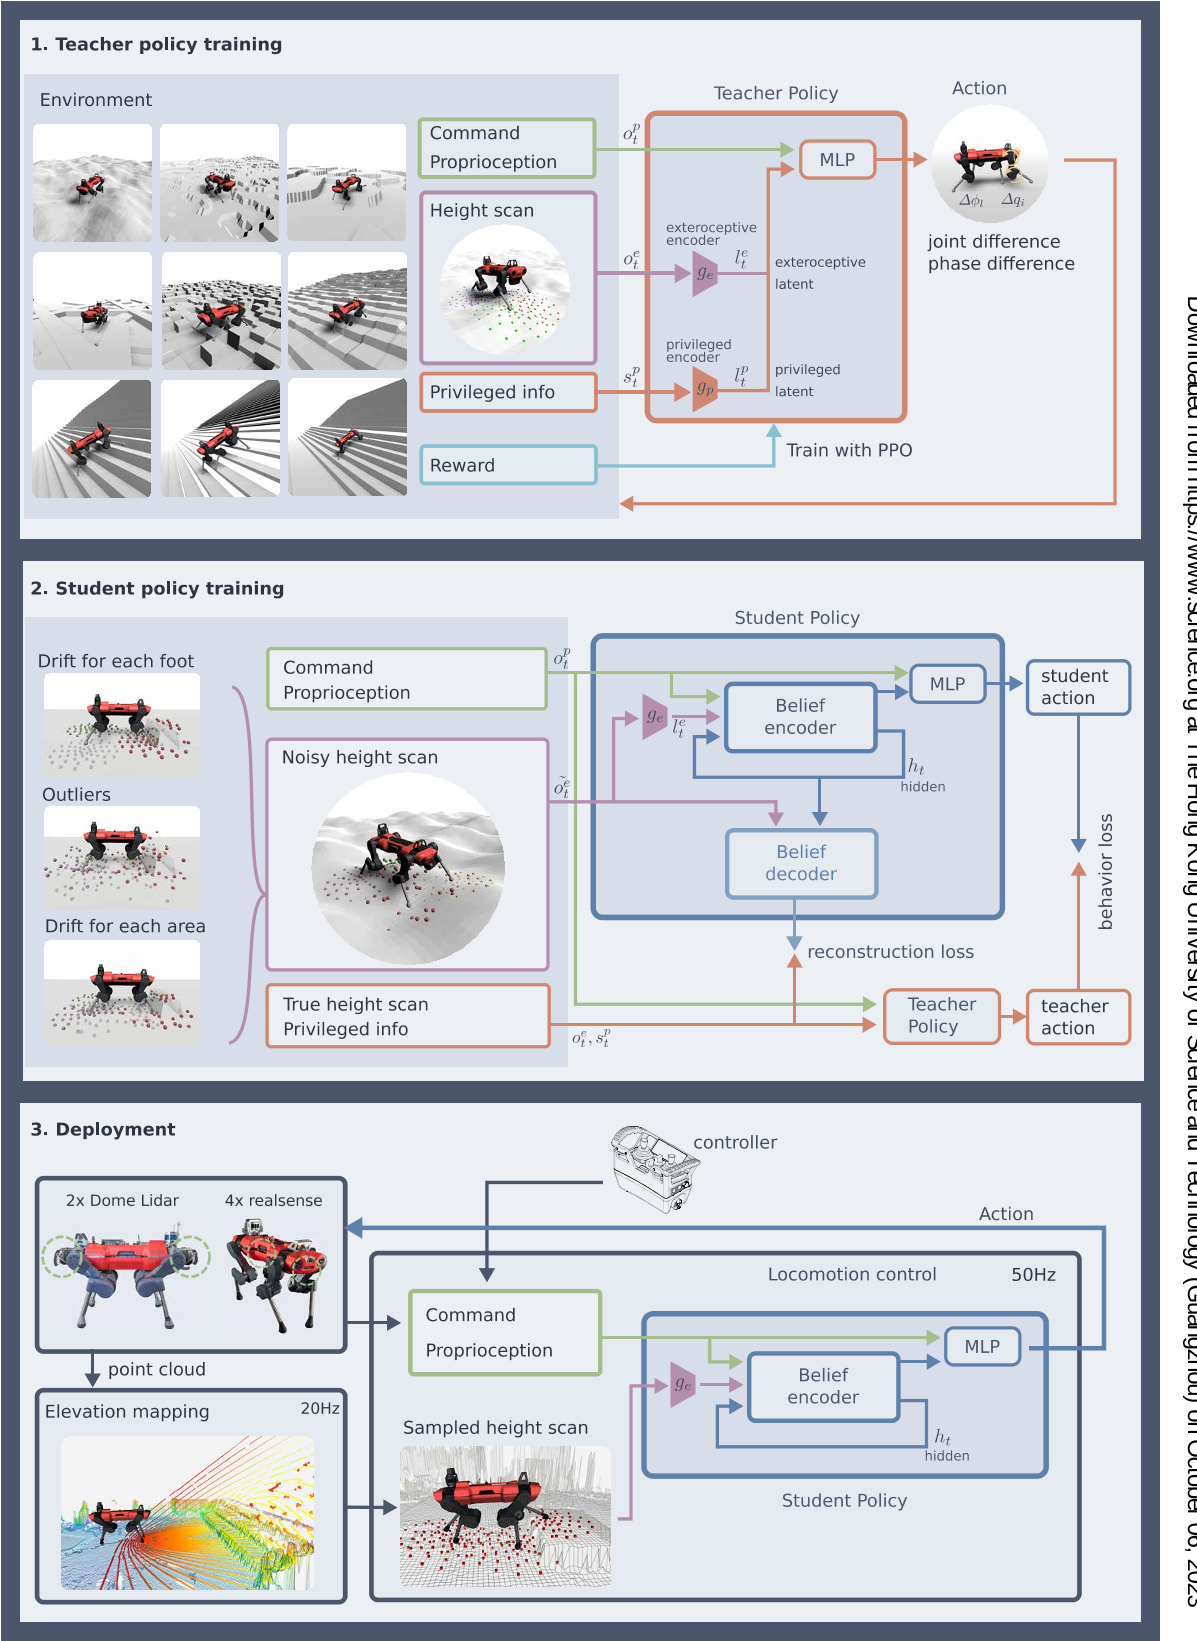
\includegraphics[width=1.0\linewidth]{train_process.png}
    \caption{RL implementation process\cite[p9]{Miki_Lee_Hwangbo_Wellhausen_Koltun_Hutter_2022}.}
    \label{fig:process}
  \end{figure}
  
  % \textcolor{gray}{\small 这节主要参考文献\cite[p10-12]{Miki_Lee_Hwangbo_Wellhausen_Koltun_Hutter_2022}。}
  
  整个神经网络的训练是在仿真环境中完成的,然后采用\emph{zero-shot sim-to-real}的转换部署到实际的额机器人上。整个方法分为三个阶段,如图\ref{fig:process}所示。
  \begin{enumerate}
    \item 首先,使用RL训练教师策略,以在随机生成的具有随机干扰的地形上遵循随机目标速度。该策略可以访问特权信息,例如无噪声地形测量、地面摩擦和引入的扰动。
    \item 在第二阶段,训练学生策略重现教师策略的动作,而不使用这种特权信息。学生策略构造一个信念状态来使用循环编码器捕获未观察到的信息,并根据该信念状态输出一个动作。在训练期间,我们利用两个损失:\emph{行为克隆损失}和\emph{重建损失}。行为克隆损失旨在模仿教师策略。重新构造损失鼓励编码器产生信息丰富的内部表示。
    \item 最后,我们将学习到的学生策略转移到物理机器人上,并将其与机载传感器在现实世界中部署。机器人通过整合来自板传感器的深度数据和从构建的高程图中采样高度读数来构建高程图,以形成策略的外部感知输入。这种外部感知输入与本体感觉数据相结合,并提供给神经网络,该网络产生执行器命令。\emph{板上传感器和自身构建等高图融合}
  \end{enumerate}
  
  \subsection[问题描述]{问题描述}
  
  我们在离散时间动力学中制定了我们的控制问题,其中环境完全由时间步$t$的状态$s_t$定义。该策略实施一个动作$a_t$并且从环境中获得一个观测结果$o_t$,这个测量结果来自观测模型$\mathcal{O}(o_t|s_t,a_t)$。接着环境以$P(s_{t+1}|s_t, a_t)$的概率转移到下一个状态$s_{t+1}$并给出一个奖励$r_{t+1}$。
  
  当所有状态都可以被观测的实况下,也即$o_t=s_t$时,整个问题可以被看做一个马尔可夫决策过程\emph{Markov decision process(MDP)}。然而,当存在不可观察性的信息时,例如外力或完整的地形信息,动力学被建模为部分可观察的马尔可夫决策过程\emph{partially observable Markov decision process(POMDP)}。
  
  RL的目标是找到一个能够使得未来轨迹的预期折扣奖励最大化的策略$\mathbfit{\pi}^*$,以使得:
  \begin{align}
    \mathbfit{\pi}^*=\underset{a}{argmax}E[\sum_{t=0}^{\infty}\gamma^t r_t]
  \end{align}
  
  已经开发了许多RL算法来解决完全可观察的MDP问题,并且易于用于训练。然而,POMDP问题的情况更具挑战性,因为状态不能完全观察到。这通常通过从历史的观察结果$o_0, \cdots, o_t$中构建一个信念状态$b_t$\emph{belief state}以尝试构建完全状态的方式来解决。在深度RL中,这通常是通过堆叠一系列先前的观察结果\cite[p]{Mnih_Kavukcuoglu_Silver_Graves_Antonoglou_Wierstra_Riedmiller_2013}或使用可以压缩过去信息的架构来完成的,例如循环神经网络 (RNN) \cite[p]{Zhu_Li_Poupart_Miao_2017}或时间卷积网络\cite[p]{Lee_Hwangbo_Wellhausen_Koltun_Hutter_2020,Bai_Kolter_Koltun_2018}。
  
  从头开始训练一个天真地处理序列数据的复杂的神经网络策略可能很耗时\cite[p]{Lee_Hwangbo_Wellhausen_Koltun_Hutter_2020}。因此,我们使用特权学习(45),我们首先训练一个具有特权信息的教师策略,然后通过监督学习将教师策略提炼为学生策略\cite[p]{Chen_Zhou_Koltun_Krähenbühl_2019}。
  
  \begin{enumerate}
    \item 训练环境:
    \item 地形:
    \item 域随机化:
    \item 片段终止条件:
  \end{enumerate}
  
  \subsection[教师策略训练]{教师策略训练}
  
  在训练的第一阶段,我们的目标是找到一个可以访问完美、特权信息的最佳参考控制策略,并使ANYmal在随机生成的地形上遵循所需的命令速度。命令需求随机生成并构成一个向量$\mathbfit{v}_des\in \mathbb{R}^3=(v_x,v_y,w)$,其中$v_x, v_y$分别表示在机器人自身坐标系下的纵向速度和横向速度,$w$表示自转速度。
  
  我们采用近端策略优化\emph{proximal policy optimization(PPO)}\cite[p]{Schulman_Wolski_Dhariwal_Radford_Klimov_2017}来训练教师策略。教师策略被建模为一个高斯策略,$a_t \sim \mathcal{N}(\pi_{\theta}(o_t=s_t),\sigma I)$,其中$\pi_{\theta}$由用$\theta$参数化的多层感知器\emph{multilayer perceptron(MLP)}实现,$\sigma$表示每个动作之间的方差。
  
  \subsection[观测和行动]{观测和行动}
  
  教师策略的观察定义为$o_t^{teacher}=(o_t^p, o_t^e, s_t^p)$,其中$o_t^p$表示本体感觉观察\emph{proprioception observation},$s_t^e$表示外部观察\emph{exteroceptive observation},$s_t^p$表示特权状态\emph{privileged state}。
  \begin{itemize}
    \item $o_t^p$包含本体速度、转动、节点位置和速度历史、动作历史、每条腿的相位;
    \item $o_t^e$是每只脚周围高度样本的向量,包括五种不同的半径;
    \item $s_t^p$包括接触状态、接触力、接触法线、摩擦系数、大腿和小腿接触状态、施加到身体上外部力和力矩、摆动阶段持续时间;
  \end{itemize}
  
  我们的动作空间受到中心模式生成器的启发\cite[p]{Lee_Hwangbo_Wellhausen_Koltun_Hutter_2020}。每条腿$l={1,2,3,4}$保存一个相位变量$\phi_l$并定义了基于相位的标称轨迹。这个标称轨迹是一个脚尖的步进运动,我们使用逆运动学来计算每个关节执行器$i={1, \dots, 12}$的标称关节目标$q_i(\phi_l)$。来自策略的动作是相差$\Delta \phi_l$和关节位置目标残差$\Delta q_i$。
  
  \sout{\textcolor{red}{\small 更详细相关内容看相关附件的S5。}}
  
  观测向量定义如\ref{tb:observations}表所示。本体感知包括命令、节点、身体信息、腿部相位信息。中央模式生成器\emph{central pattern generator(CPG)}的相位信息包含$\Delta\phi_l, \cos\phi_l, \sin\phi_l$和每条腿$l$的基础频率。对于外部感知我们采用每个脚周围的高度采样来代替局部高程图。圆形采样模式包括每只脚周围的$\{6, 8, 10, 12, 16\}$个点,半径分别为$\{0.08, 0.16, 0.26, 0.36, 0.48\}$m。
  
  运动被定义为$\langle \Delta \phi_l, \Delta q_i \rangle$,其中$\Delta \phi_l$和$\Delta q_i$分别表示每个条腿($l\in\{legs\}$)的相位偏移和节点目标位置残差($i\in \{1, \dots, 12\}$)。
  我们有一个标称轨迹$\mathbfit{p}(\phi):\mathbb{R}\longrightarrow\mathbb{R}^3$,它将各个$\phi_l$映射到目标脚位置,随着$\phi$在$[0,2\pi)$范围内生成周期性步进运动。从动作中,每条腿$l$的节点目标位置用逆运动学$IK(\cdot)$和基础相位频率$\Delta\phi_0$定义为$q_{i\in l}^{target}=IK(\mathbfit{p}(\phi_l+\Delta \phi_l + \Delta \phi_0))+\Delta q_{i\in l}$。
  
  标称足迹定义如下。如果相位是处于上摆动期间($0\leq\phi_l\leq \pi/2$)则:
  \begin{align}
    \mathbfit{p}_l(\phi_l)=\langle x_l^n, y_l^n, z_l^n + 0.2\cdot(-2t_l^3+3t_l^2)\rangle, where\ t_l=2/\pi\cdot\phi_l
  \end{align}
  
  $\{x,y,z\}_l^n$是默认姿态配置处的标称脚位置。三次Hermite样条在$\phi_l=0$处连接$z=z_l^n$在$\phi_l=\pi/2$处连接$z=z_l^n+0.2$。
  
  在下摆动期间($\pi/2 < \phi_l \leq \pi$),足高计算如下:
  \begin{align}
    \mathbfit{p}_l(\phi_l)=\langle x_l^n, y_l^n, z_l^n + 0.2\cdot(2t_l^3-3t_l^2+1)\rangle, where\ t_l=2/\pi\cdot\phi_l-1
  \end{align}
  
  它与前面的函数对称。在驻立阶段($\pi< \phi_l \leq 2\pi$),$\mathbfit{p}_l(\phi_l)=\langle x_l^n, y_l^n, z_l^n \rangle$。
  
  
  
  \begin{table}
    \centering
    \caption{Observations. Proprioception is used for both teacher and student training. Exteroception is given in the form of height samples. The privileged information is used only for teacher training.}
    \label{tb:observations}
    \begin{tabular}{l|ll}
      \hline
      Observation type & Input & Dimensionality\\
      \hline
      \multirow{9}{*}{Proprioception} & command & 3\\
      &body orientation & 3\\
      &body velocity & 6 \\
      &joint position & 12 \\
      &joint velocity & 12 \\
      &joint position history (3 time steps) & 36\\
      &joint velocity history (2 time steps) & 24 \\
      &joint target history (2 time steps) & 24 \\
      &CPG phase information & 13 \\
      \hline
      Exteroception & height samples & 208\\
      \hline
      \multirow{8}{*}{Privileged info.} & contact states & 4\\
      &contact forces & 12\\
      &contact normals & 12 \\
      &friction coefficients & 4\\
      &thigh and shank contact & 8 \\
      &external forces and torques & 6\\
      &airtime & 4 \\
      \hline 
    \end{tabular}
  \end{table}
  
  
  \subsection[策略构架]{策略构架}
  
  我们将教师策略$\pi_{\theta}$建模为一个MLP。它包括三个MLP组成部分:外部感知编码器、特权编码器、主网络,如图\ref{fig:process}所示。
  \begin{enumerate}
    \item 外部感知编码器$g_e$接收来自$o_t^e$的信息,然后输出一个小些的潜在表示$$l_t^e=g_e(o_t^e)$$
    \item 特权编码器$g_p$接收来自特权状态$s_t^p$的信息,然后输出一个潜在表示$$l_t^{priv}=g_p(s_t^p)$$
    \item 
  \end{enumerate}
  
  这些编码器将每个输入压缩为更紧凑的表示,并使得学生策略能更方便地重用一些教师策略组件。
  
  \sout{\textcolor{red}{\small 更详细相关内容看相关附件的S6。}}
  
  策略网络由多层MLP组成。用基于MLP的编码器$(g_e,g_p)$,将高度采样结果首先编码成为一个$24\times4=96$维的潜在向量;将特权信息编码成为一个$24$维的潜在变量。每个编码器有两层分别是$\{80,60\}$和$\{64,32\}$的隐藏单元。高度样本首先分别针对每只脚分别输入到编码器中,然后连接成一个特征向量。然后将这些特征与本体感受观察连接起来,并馈送到另一个具有三个隐藏层$\{256, 160, 128\}$的MLP。所有MLP的激活函数为LeakyReLU (72)。
  
  我们使用具有外部感受门的GRU作为信念编码器(图\ref{fig:terrain_perception}C)。GRU由2个堆叠的层组成,每个层有$50$个隐藏单元。
  信念编码器和外部感知门$g_b,g_a$用于计算$96 + 24 = 120$维信念状态$b_t$和$96$维注意力向量$\alpha$。每个编码器有两个隐藏层,每个隐藏层有$\{64, 64\}$和$\{64, 64\}$个隐藏单元。过滤后的外部感受信息$l_t^e\odot\alpha$被添加到$g_b(b_t')$,使用零填充来匹配维度差异。
  
  \subsection[奖励函数]{奖励函数}
  
  针对速度控制命令的跟随,我们定义正奖励;针对违反约束的情况,我们定义负奖励。指令跟随奖励定义如下:
  \begin{align}
    \mathbfit{r}_{command}=\begin{cases}
      1.0, &if \mathbfit{v}_{des}\cdot\mathbfit{v}>|\mathbfit{v}_{des}|\\
      \exp(-(\mathbfit{v}_{des}\cdot\mathbfit{v})^2), &otherwise
    \end{cases}
  \end{align}
  
  其中$\mathbfit{v}_{des}\in\mathbb{R}^2$是所需的水平速度,$\mathbfit{v}\in\mathbb{R}^2$是身体坐标系下当前身体速度。同样的奖励机制也被应用与转动速度情况。
  
  我们惩罚与期望速度正交的速度分量以及横摇、俯仰和偏航周围的身体速度。此外,我们使用整形奖励进行身体方向、关节扭矩、关节速度、关节加速度和脚滑以及小腿和膝盖碰撞。身体方向奖励用于避免身体的奇怪姿势。联合相关奖励术语用于避免过于激进的运动。脚滑和碰撞奖励术语用于避免它们。我们通过在模拟中查看策略的行为来调整奖励术语。除了遍历性能外,我们还检查了运动的平滑度。
  
  \sout{\textcolor{red}{\small 更详细相关内容看相关附件的S7。}}
  
  奖励函数定义为:
  \begin{align}
    r=0.75(r_{lv}+r_{av}+r_{lvo})+r_b+0.003r_{fc}+0.1r_{co}+0.001r_j+0.08r_{jc}+0.003r_s+1.0\cdot 10^{-6}r_{\tau}+0.003r_{slip}
  \end{align}
  各项的具体定义如下:
  \begin{enumerate}
    \item 线速度奖励\emph{Linear Velocity Reward($r_{lv}$)}:这项鼓励策略去跟随需要的水平($x,y$ plane)速度指令:\begin{align}
      r_{lv}=\begin{cases}
      \exp(-|\mathbfit{v}|^2), & if |\mathbfit{v}_{des}|=0\\
      1.0, & else if \mathbfit{v}_{des}\cdot\mathbfit{v}>|\mathbfit{v}_{des}|\\
      \exp(-(\mathbfit{v}_{des}\cdot\mathbfit{v}-|\mathbfit{v}_{des}|)^2), & otherwise
    \end{cases}
    \end{align}其中$\mathbfit{v}_{des}\in\mathbb{R}^2$是目标水平速度,$\mathbfit{v}\in\mathbb{R}^2$是身体坐标系下当前身体的速度。
    \item 角速度奖励\emph{Angular Velocity Reward($r_{av}$)}:这一项鼓励策略去跟随需要的转动速度指令:\begin{align}
      r_{av}=\begin{cases}
      \exp(-w_z^2), & if w_{des}=0\\
      1.0, & else if w_{des}\cdot\mathbfit{w}_z>w_{des}\\
      \exp(-(w_{des}\cdot w_z-|w_{des}|)^2), & otherwise
    \end{cases}
    \end{align}
    \item 线性正交速度奖励\emph{Linear Orthogonal Velocity Reward($r_{lvo}$)}:这项惩罚与目标速度指令正交的速度:\begin{align}
      r_{lvo}=\exp(-3.0|\mathbfit{v}_o|^2), where\ \mathbfit{v}_o=\mathbfit{v}-(\mathbfit{v}_{des}\cdot\mathbfit{v})\mathbfit{v}_{des}
    \end{align}
    \item 身体运动奖励\emph{Body Motion Reward($r_{b}$)}:这项惩罚身体速度中不符合指令要求的部分:\begin{align}
      r_{bm}=-1.25v_z^2-0.4|\omega_x|-0.4|\omega_y|
    \end{align}
    \item 脚感奖励\emph{Foot Clearance Reward($r_{fc}$)}:当一条腿处于摆动相位时,比如$\phi_i\in[0,\pi)$,机器人应该将这条腿上对应的脚抬起到比障碍物高的程度。但是,为了防止机器人做出不必要的抬高间隙,我们通过给出惩罚$r_{fcl}$来正则化腿轨迹。$H_{sample,l}$是第$l$只脚的高度采样。这样,间隙成本定义为:\begin{align}
      &f_{fcl}=
      \begin{cases}
      -1.0, & if\ \max(H_{sample,l})<-0.2\\
      0.0, &otherwise\\
      \end{cases}\\
      &r_{fc}=\sum_{l=1}^{4}r_{fcl}
    \end{align}注意高度样本是相对于脚高度进行采样,因此$-0.2$表示地形高度比脚低$0.2$m;脚比采样的地形高度高$0.2$m。
    \item 小腿和膝关节碰撞奖励\emph{Shank and Knee Collision Reward($r_{co}$)}:我们希望惩罚脚以外的地形和机器人部件之间的不良接触,以避免硬件损坏:$$r_{co}=\begin{cases}
      -c_k, & if\ shank\ or\ knee\ is\ in\ collision\\
      0.0, & otherwise\\
    \end{cases}$$这里$c_k$是课程因子,它单调增加并收敛到1。
    \item 节点运动奖励\emph{Joint Motion Reward($r_{j}$)}:该项惩罚关节速度和加速度以避免振动:\begin{align}
      r_s=-c_k\sum_{i=1}^{12}(0.01\dot q_i^2+\ddot q_i^2)
    \end{align}其中$\dot q_i, \ddot q_i$分别是节点的速度和加速度。
    \item 节点约束奖励\emph{Joint Constraint Reward($r_{jc}$)}:该项在联合空间中引入了一个软约束。为了避免相反方向的膝关节翻转,我们对超过阈值的惩罚:\begin{align}
      r_{jc,i}=\begin{cases}
        -(q_i-q_{i,th})^2, & if\ q_i>q_{i,th}\\
        0.0, & otherwise\\
      \end{cases}\\
      r_{jc}=\sum_{i=1}^{12}r_{jc,i}\\
    \end{align}其中$q_{i,th}$是第$i$个节点的阈值。我们只设置膝关节的阈值。
    \item 目标平滑奖励\emph{Target Smoothness Reward($r_{s}$)}:通过对目标位置一阶和二阶有限差分导数的大小进行惩罚,使生成的足部轨迹变得更平滑:\begin{align}
      r_s=c_k\sum_{i=1}^{12}((q_{i,t}^{des}-q_{i,t-1}^{des})^2+(q_{i,t}^{des}-2q_{i,t-1}^{des}+q_{i,t-2}^{des})^2)
    \end{align}其中$q_{i,t}^{des}$是$t$步时间里第$i$个节点的目标位置。
    \item 扭矩奖励\emph{Torque Reward($r_{\tau}$)}:我们惩罚节点的扭矩里节省能耗($\tau\propto electric current$):\begin{align}
      r_{\tau}=-c_k\sum_{i=1}^{12}\tau_i^2
    \end{align}其中$\tau_i$是执行器网络计算出的第$i$个节点的扭矩。
    \item 滑动奖励\emph{Slip Reward($r_{slip}$)}:我们惩罚与地面接触的脚的速度以减少滑动情况:\begin{align}
      r_{slip}=-c_k\sum_{l\in \{foot in contact\}}v_{f,l^2}
    \end{align}其中$v_{f,l^2}$是与地面接触了的第$l$只脚的速度。
  \end{enumerate}
  \subsection[课程]{课程}
  随着策略性能的提高,我们使用两个课程来提高难度。
  一个课程使用自适应方法\cite[p]{Lee_Hwangbo_Wellhausen_Koltun_Hutter_2020}调整地形难度,另一个改变元素,如奖励或使用逻辑函数\cite[p]{Hwangbo_Lee_Dosovitskiy_Bellicoso_Tsounis_Koltun_Hutter_2019}应用干扰。
  
  对于地形课程,粒子滤波更新地形参数,使它们仍然具有挑战性,但在策略训练期间的任何时候都可以实现\cite[p]{Lee_Hwangbo_Wellhausen_Koltun_Hutter_2020}。
  
  第二个课程将域随机化的幅度和一些奖励项(关节速度、关节加速度、方向、滑移和大腿和小腿接触)乘以单调递增且渐近趋势为 1 的因子:$$c_{k+1}=(c_k)^d$$
  
  其中$c_k$是第$k$次迭代的课程因子,$d\in(0,1)$是收敛率。
  
  \subsection[学生策略训练]{学生策略训练}
  
  在我们训练好一个可以在特权信息的帮助下穿越各种地形教师策略后,我们就可以将其提炼成一个学生策略,该策略只能访问真实robot上可用的信息。我们使用与教师策略相同的训练环境,但在学生高度样本观察中添加额外的噪声:$o_t^{student}=(o_t^p,n(o_t^e))$,其中$n(o_t^e)$是一个用于高度样本输入的噪声模型。该噪声模型模拟了现场部署过程中经常遇到的外部感觉的不同失败案例,具体如下。
  
  当外部感觉中存在较大的噪声时,它变得不可观察;因此,动力学被认为是POMDP。此外,由于缺乏直接测量的传感器,特权状态是不可观察的。因此,该策略需要考虑顺序相关性来估计不可观察的状态。我们建议使用\emph{循环信念状态编码器}来组合外部感知和本体感觉的序列,以估计不可观察的状态作为信念状态。
  
  学生策略由循环信念状态编码器和MLP组成,如图\ref{fig:process}所示。我们用$h_t$表示循环网络的隐藏状态。信念状态编码器接收$o_t^{sutdent},h_t$并输出一个潜在向量$b_t$,它表示信念状态。我们的目标是将信念状态$b_t$与编码所有运动相关信息的教师策略的特征向量($l_t^e, l_t^{priv}$)进行匹配。
  接下来我们将$o_t^p$和$b_t$传入MLP,由它计算出最终的动作。MLP结构与教师策略相同,这样我们就可以重用教师策略的学习权重来初始化学生网络并加快训练速度。
  
  学生策略的训练通过最小化两个损失以有监督的方式进行训练:行为克隆损失\emph{behavior cloning loss}和重建损失\emph{reconstruction loss}。
  \begin{itemize}
    \item 克隆损失定义为给定相同状态和指令的学生动作和教师动作之间的平方距离。
    \item 重建损失定义为无噪声高度样本和特权信息($o_t^e, s_t^p$)及其与信念状态$b_t$的重建之间的平方距离。
  \end{itemize}
  
  我们通过推出学生策略来生成样本,以提高鲁棒性\cite[p]{Ross_Gordon_Bagnell_2010,Czarnecki_Pascanu_Osindero_Jayakumar_Swirszcz_Jaderberg_2019}。
  
  \subsection[高度采样随机化]{高度采样随机化}
  
  \begin{figure}
    \centering
    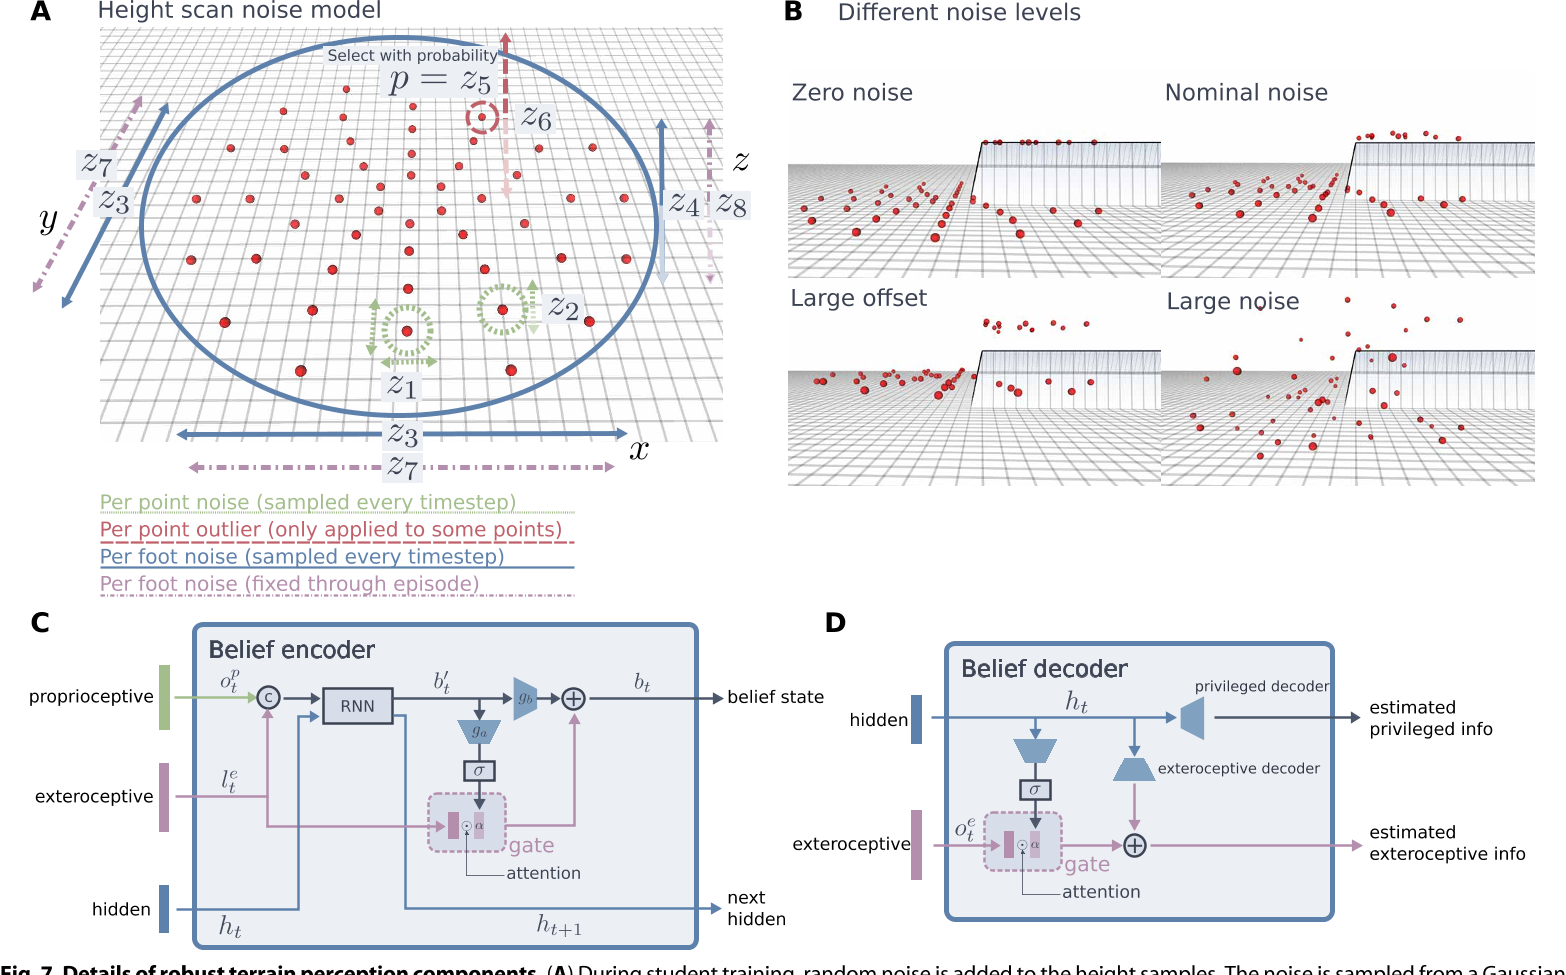
\includegraphics[width=1.0\linewidth]{terrain_perception.png}
    \caption{Robust terrain perception\cite[p10]{Miki_Lee_Hwangbo_Wellhausen_Koltun_Hutter_2022}.}
    \label{fig:terrain_perception}
  \end{figure}
  
  在学生训练过程中,我们使用参数化噪声模型$n(\sigma_t^e|o_t^e,z),z\in \mathbb{R}^{8\times 4}$将随机噪声注入到高度样本中。
  我们在对高度进行采样时应用了两种不同类型的测量噪声,如图\ref{fig:terrain_perception}A所示:
  \begin{enumerate}
    \item 横向移动扫描点。
    \item 扰动高度值。
  \end{enumerate}
  
  每个噪声值都是从高斯分布中采样的,噪声参数$z$定义方差。这两种类型的噪声都应用于三个不同的范围,所有这些都有自己的噪声方差:每个扫描点、每只脚和每一集。每个扫描点和每只脚的噪声值在每个时间步重新采样,而所有扫描点的表观轮廓噪声保持不变。
  
  此外,我们定义了三个具有相关噪声参数$z$的映射条件来模拟不断变化的地图质量和误差源,如图\ref{fig:terrain_perception}B所示。
  \begin{enumerate}
    \item 名义噪声假设常规操作期间具有良好的地图质量。
    \item 大偏移量噪声来模拟由于姿态估计漂移或可变形地形造成的地图偏移。
    \item 幅度较大的噪声来模拟由于遮挡或映射失败导致完全缺乏地形信息的情况。
  \end{enumerate}
  
  这三个映射条件在每个训练集的开头以60\%、30\%和10\%的比例选择。
  
  最后,我们将每个训练地形划分为单元格,并向高度样本添加附加偏移量,具体取决于它采样的单元格。这模拟了不同地形特征的区域之间的转换,如植被和深度雪。参数向量$z$也是学习课程的一部分,其幅度随训练持续时间线性增加。
  
  \sout{\textcolor{red}{\small 更详细相关内容看相关附件的S8。}}
  
  在学生训练期间,我们随机化每只脚周围绘制的高度样本(图\ref{fig:terrain_perception}A)。我们扰动每个样本的位置,并将噪声添加到测量的高度值中,如下所示。
  \begin{align}
    x_p=r_p\cos(\theta_p)+\epsilon_{px}+\epsilon_{fx}+w_x\\
    y_p=r_p\sin(\theta_p)+\epsilon_{py}+\epsilon_{fy}+w_y\\
    h_p=h(x_p,y_p)+\epsilon_{pz}+\epsilon_{fz}+w_z+\epsilon_{outlier}
  \end{align}
  
  其中$h(x_p,y_p)$表示在点$(x_p,y_p)$处的高度,$r_p$是$p$点的径向距离,$\theta_p$是$p$在脚周围的极坐标中的方位角。$\epsilon_{px},\epsilon_{py},\epsilon_{pz}$表示每个时间步长里各个点的采样噪声。$\epsilon_{fx},\epsilon_{fy},\epsilon_{fz}$表示每个时间步长里各个脚的采样噪声。$w_x, w_y, w_z$表示每个片段里各个脚的采样噪声。$\epsilon_{outlier}$是间歇性添加的大噪声来模拟异常值。
  
  使用参数$z$从正态分布中采样每个噪声。$\epsilon_{px},\epsilon{py}\sim \mathcal{N}(0,z_0), \epsilon{pz}\sim \mathcal{N}(0,z_1), \epsilon_{fx},\epsilon{fy}\sim \mathcal{N}(0,z_2), \epsilon{fz}\sim \mathcal{N}(0,z_3), \epsilon_{outlier}\sim \mathcal{N}(0,z_4)$ 概率分别为 $p=z_5,w_x,w_y\sim\mathcal{N}(0,z_6),w_z\sim\mathcal{N}(0,z_7)$。
  
  我们为学生训练定义三种情况:\emph{nominal, offset, noisy}。每种情况的参数$z$定义如下:
  \begin{align}
    z_{nominal}=\langle0.004, 0.005, 0.01, 0.04, 0.03,0.05, 0.1\rangle\\
    z_{offset}=\langle0.004, 0.005, 0.01, 0.1c_{sk}, 0.1c_{sk},0.02, 0.1\rangle\\
    z_{noisy}=\langle0.004, 0.1c_{sk}, 0.1c_{sk}, 0.3c_{sk}, 0.3c_{sk},0.3c_{sk}, 0.1\rangle
  \end{align}
  
  其中$c_{sk}$是学生课程因子,会随着训练片段增加而不断线性增加。
  我们在轨迹的开头和中间随机选择其中一个条件。选择的概率分别是60\%、30\%和10\%。
  
  
  \subsection[信念状态寄存器]{信念状态寄存器}
  
  循环信念状态编码器编码不能直接观察到的状态。为了整合本体感受和外感受数据,我们引入了一个门控编码器,如图 7C 所示,灵感来自门控 RNN 模型\cite[p]{Cho_van_Merrienboer_Gulcehre_Bahdanau_Bougares_Schwenk_Bengio_2014, Hochreiter_Schmidhuber_1997}和多模态信息融合 (4-66)。
  
  信念状态编码器学习使用一个可变的门控因子来控制外部感知信息通过的量。首先,内部感知$s_t^p$、从含噪声观测提取的外部感知$l_t^e=g_e(\widetilde o_t^e)$以及隐藏状态$s_t$被RNN模型编码成为一个中间信念状态$b_t{t'}$。它控制最终进入$b_t$的外部感知信息量:
  \begin{align}
    b_{t'},h_{t+1}=RNN(o_t^p,l_t^e,h_t)\\
    \alpha = \sigma (g_a(b_{t'}))\\
    b_t = g_b(b_{t'})+l_t^e \odot \alpha
  \end{align}
  
  这里$g_a,g_b$是全连接的神经网络,$\sigma(\cdot)$是sigmoid函数。
  
  解码器使用相同的门,用于重建特权信息和高度样本(图 7D)。这用于计算重建损失,它鼓励信念状态捕获有关环境的真实信息。我们使用 GR\cite[p]{Cho_van_Merrienboer_Gulcehre_Bahdanau_Bougares_Schwenk_Bengio_2014}作为我们的 RNN 架构。
  
  \sout{\textcolor{red}{\small 门结构有效性的评估见第 S9 节。}}
  
  \subsection[部署]{部署}
  
  我们在 PyTorch\cite[p]{Paszke_Gross_Massa_Lerer_Bradbury_Chanan_Killeen_Lin_Gimelshein_Antiga_et_al_2019}中训练策略,并在没有任何微调的情况下部署在机器人 zero-shot上。我们通过估计机器人的姿态,并相应地从传感器中调节点云读数,构建了一个以机器人为中心的2.5D高程图刷新率为20赫兹。该策略以50Hz运行,并从最新的高程图中映射采样高度;如果查询位置没有可用的地图信息,则填充随机采样的值。
  
  我们开发了一个高程映射管道,用于在图形处理单元上快速地形映射,以并行化点云处理。我们遵循与Fankhauser等人\cite[p]{Fankhauser_Bloesch_Hutter_2018}使用的类似方法,以卡尔曼滤波的方式更新地图,另外按漂移补偿\emph{drift compensation}和光线投射\emph{ray casting}以获得更吻合的地图。这种快速映射实现对于保持快速处理速率和跟上我们的控制器实现的快速运动速度至关重要。
  
  


\section[电机驱动关节点模型]{电机驱动关节点模型\cite[p4]{Gehring_Coros_Hutter_Bellicoso_Heijnen_Diethelm_Bloesch_Fankhauser_Hwangbo_Hoepflinger_et_al_2016}}

\textcolor{red}{\small
基于参考文献阐述\emph{电机驱动关节点模型}描述...
}
